\clearpage
\section{核心逻辑}

\subsection{初始化 SwornDisk Device Mapper 目标设备}

\mintinline{text}{DmSwornDiskHandler::ctr (dm-sworndisk/src/handler.rs:28)}

初始化并创建 SwornDisk 虚拟块设备通过 \mintinline{text}{dmsetup} 命令完成,执行该命令时会触发 SwornDisk 的 \mintinline{c}{dm_ctr_fn} (constructor) 回调函数。在 ctr 函数中,主要做的事情是向系统注册 SwornDisk 虚拟块设备、读取或创建 SwornDisk 的关键数据结构,初始化 SwornDisk 的上下文对象。具体地来说:

\begin{itemize}[itemsep=2pt,topsep=0pt,parsep=0pt]
  \item 解析 dmsetup 的参数,获取数据磁盘和元数据磁盘的设备路径
  \item 在 Device Mapper 的 table 中注册设备
  \item 从 meta device 中读取或初始化超级块、Checkpoint
  \item 创建数据段缓冲区、索引段实例、MemTable、工作队列和 bio 处理队列等
  \item 创建 BIT 缓存
  \item 将所有在 SwornDisk 生命周期所需用到的结构与对象包装到 SwornDiskContext 中
\end{itemize}

\subsection{卸载 SwornDisk Device Mapper 目标设备}

\mintinline{text}{DmSwornDiskHandler::dtr (dm-sworndisk/src/handler.rs:175)}

从系统的 Device Mapper table 中释放 SwornDisk 注册的虚拟块设备。

\subsection{处理 bio}

\mintinline{text}{DmSwornDiskHandler::map (dm-sworndisk/src/handler.rs:191)}

SwornDisk Linux Rust 目前实现了三种磁盘 I/O 请求的处理:\textbf{读 (READ)、写 (WRITE)、刷盘 (FLUSH)}. 

\begin{itemize}[itemsep=2pt,topsep=0pt,parsep=0pt]
  \item 当有上述三种类型的 bio 请求到达时,将会首先调用 SwornDisk 的 \mintinline{text}{dm_map_fn} 函数进行处理,将其加到 \mintinline{rust}{SwornDiskContext} 中的 bio 队列 \mintinline{rust}{ctx.bio_queue}  中。这是一个全局共享的 bio 队列,因此对其进行读取或修改前需要先加锁。
  \item 将处理 I/O 的 worker \mintinline{rust}{crate::workers::IoWorker} 加入全局 CMWQ 中(同一个 worker 只会被加入到工作队列一次)。
  \item 返回 \mintinline{rust}{DM_MAPIO_SUBMITTED} 状态码或 \mintinline{rust}{DM_MAPIO_KILL} 状态码(如果 bio 的类型未被支持)。
\end{itemize}

将 bio 加入队列之后,后续对 bio 的处理逻辑均在 \mintinline{rust}{IoWorker} 中完成:\mintinline{text}{dm-sworndisk/src/workers/io.rs:12}.

\subsection{写入数据}

\mintinline{text}{IoWorker::handle_write_request (dm-sworndisk/src/workers/io.rs:160)}

处理写入请求的步骤:

\begin{itemize}[itemsep=2pt,topsep=0pt,parsep=0pt]
  \item 首先计算 bio 请求的扇区号所对应的 LBA 范围;
  \item 根据 LBA 将 bio 的数据拆成若干个块大小的分片;
  \item 对于每个 LBA 及其对应的数据分片,将数据以明文形式写入 SwornDiskContext 中的数据段缓冲区中 \mintinline{rust}{ctx.data_seg_buffer},并维护 LBA 与数据的对应关系。
  \item 写入时会首先更新 Checkpoint 中的 DST,分配一个新的可用块。如果当前 LBA 的记录已存在,执行原地更新。
  \begin{itemize}[itemsep=2pt,topsep=0pt,parsep=0pt]
    \item 如果此时数据段缓冲区已写满,则触发\textbf{将数据段缓冲区写回磁盘数据段}的操作:
    \item 对于数据段中所有 LBA 及对应的明文数据,随机生成 key, nonce 使用 AES-128-GCM 算法进行加密,并得到 MAC
    \item 将 \mintinline{text}{LBA → (HBA, key, nonce, MAC)} 的对应关系记录 (Record) 写入 MemTable 中
    \item 清空数据段缓冲区,并从 Checkpoiint 的 DST 中请求分配一个新的数据段。
  \end{itemize}
  \item 如果 MemTable 写满(Record 数量达到阈值),将触发 minor compaction
  \begin{itemize}[itemsep=2pt,topsep=0pt,parsep=0pt]
    \item 使用 MemTable 中的 Record 创建 BIT
    \item 将 BIT 根节点的信息写入 Checkpoint 的 BITCagetory 中
    \item 清空当前 MemTable
    \item 检查当前是否需要进行 major compaction, 如果需要则创建一个 compaction worker 加入工作队列中
  \end{itemize}
  \item 调用 \mintinline{rust}{bio.end()} 结束 bio 请求
\end{itemize}

\subsection{读取数据}

\mintinline{text}{IoWorker::handle_read_request (dm-sworndisk/src/workers/io.rs:60)}

处理读取请求的步骤:

\begin{itemize}[itemsep=2pt,topsep=0pt,parsep=0pt]
  \item 首先计算 bio 请求的扇区号所对应的 LBA 范围;
  \item 对于每个 LBA:
  \begin{itemize}[itemsep=2pt,topsep=0pt,parsep=0pt]
    \item 首先从数据段缓冲区中,查找是否有对应该 LBA 的明文数据,若有则直接填入 bio
    \item 接下来从 MemTable 中,查找是否有对应该 LBA 的加密信息 Record,若有则根据 Record 中的 HBA, Key, nonce 和 MAC 从磁盘数据段读入对应的块并解密,返回给 Bio
    \item 如果请求的 LBA 不在 MemTable 中,接下来按照层级有小到大、最后修改时间的逆序遍历 dsLSM-tree 中的 BIT,查找对应该 LBA 的加密信息(查找 LBA 时需要先通过 BIT 节点记录的 \mintinline{rust}{lba_range} 判断当前 LBA 是否在此 BIT 节点中,在单个 BIT 节点中查找的复杂度为 $O(\log n)$),若找到 Record 则根据其中的 HBA, Key, nonce 和 MAC 从磁盘数据段读入对应的块并解密,并返回给 bio
    \item 在从 BIT 索引的过程中,会将读到的 BIT 中间节点或叶节点,缓存到 SwornDiskContext 的 BIT 节点块缓存 (\mintinline{text}{ctx.indirect_block_cache, ctx.leaf_block_cache}) 中。
  \end{itemize}
  \item 调用 \mintinline{rust}{bio.end()} 结束 bio 请求
\end{itemize}

\subsection{BlockIndexTable (BIT) 实现}

SwornDisk Linux Rust 对 BIT 的实现是\textbf{直接在磁盘上以块为单位维护 BIT},如图\ref{swrodnsik-rust-bit}所示:

\begin{figure}[H]
  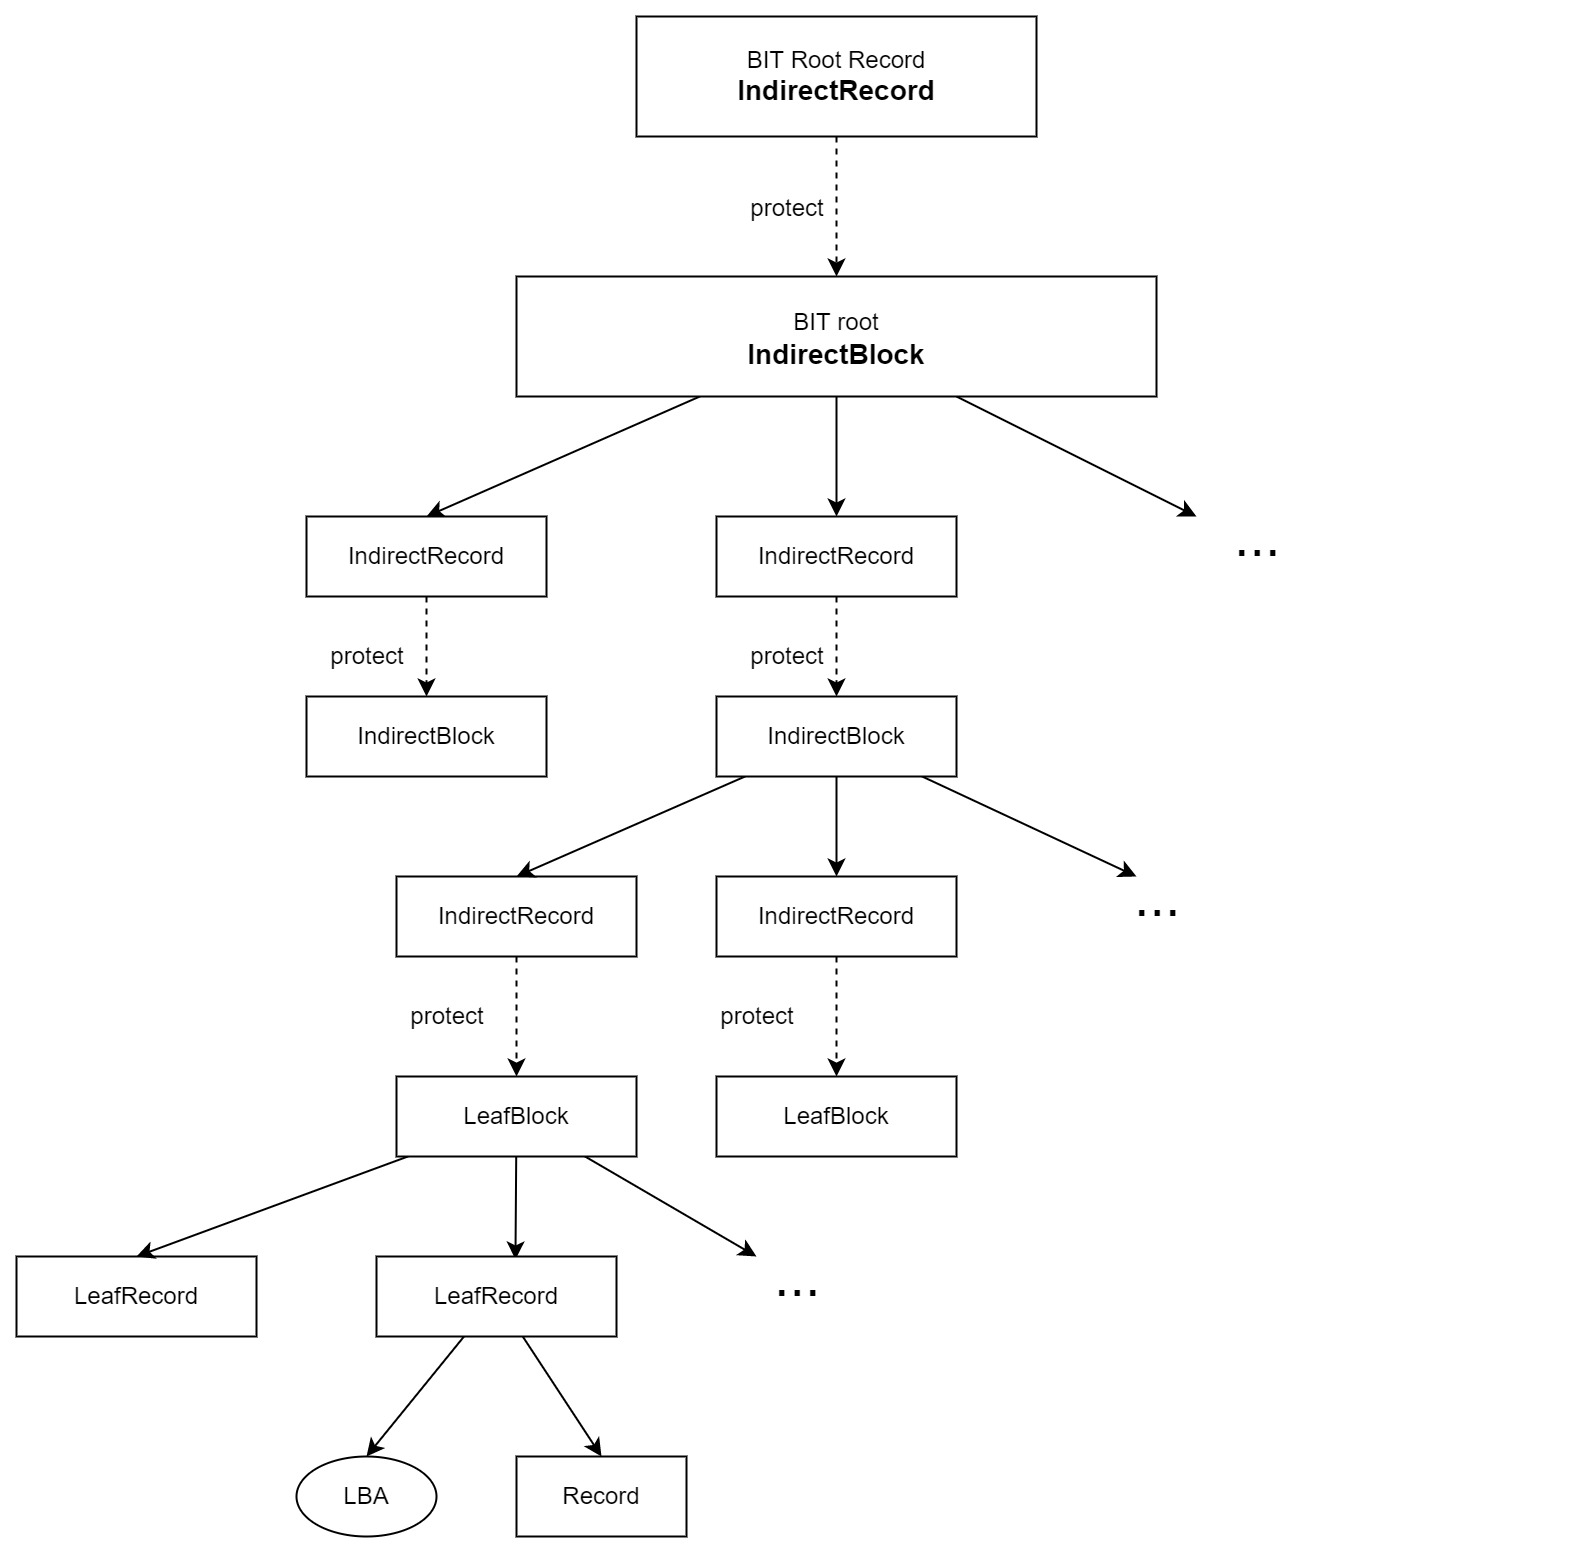
\includegraphics[width=0.8\textwidth]{images/bit-structure.jpg}
  \caption{SwornDisk Linux Rust BIT 结构}
  \label{sworndisk-rust-bit}
\end{figure}

BIT 的节点以块为单位组织,分为两类:IndirectBlock 和 LeafBlock;每个块都被 IndirectRecord 结构保护,维护了节点块的 HBA, key, MAC, nonce 和节点的 LBA 范围。

\clearpage
\subsubsection{数据结构定义}

\begin{minted}{rust}
/// BIT Record
#[derive(Copy, Clone, Debug)]
pub struct Record {
    /// HBA (Hardware Block Address)
    pub hba: u64,
    /// Crypto key
    pub key: KeyType,
    /// Crypto random string (a.k.a nonce / iv)
    pub nonce: NonceType,
    /// Crypto authentication data (a.k.a MAC / tag)
    pub mac: MacType,
}

#[derive(Copy, Clone, Debug)]
/// Leaf node of BIT
pub struct LeafRecord {
    /// logical block address of current record
    pub lba: u64,
    /// hba & key & nonce & mac
    pub record: Record,
}

#[derive(Debug)]
/// On-disk unit of leaf node
pub struct LeafBlock {
    /// number of LeafRecord
    pub count: usize,
    /// children vector
    pub children: Vec<LeafRecord>,
}

#[derive(Copy, Clone, Debug)]
/// Indirect node of BIT
pub struct IndirectRecord {
    /// lba range of IndirectBlock responding to this IndirectRecord
    pub lba_range: (u64, u64),
    /// hba & key & nonce & mac
    pub record: Record,
}

#[derive(Debug)]
/// On-disk unit of indirect node
pub struct IndirectBlock {
    /// number of IndirectRecord
    pub count: usize,
    /// children vector
    pub children: Vec<IndirectRecord>,
}

#[derive(Debug)]
pub struct BIT {
    /// root node of BIT
    pub root: IndirectBlock,

    /// IndirectRecord of root node
    pub record: IndirectRecord,

    /// max level of BIT
    pub level: usize,

    /// element number of BIT
    pub size: usize,
}
\end{minted}

\subsubsection{从 MemTable 创建 BIT}

\mintinline{text}{BIT::from_memtable (dm-sworndisk/src/regions/index/bit.rs:320)}

\begin{itemize}[itemsep=2pt,topsep=0pt,parsep=0pt]
  \item 计算 MemTable 中元素数量所需的 BIT 层级
  \item 分配 LeafBlock 和 IndirectBlock 的缓冲区
  \item 遍历 MemTable 中的 $(lba, record)$,加入 LeafBlock 中
  \item 如果 LeafBlock 或 IndirectBlock 写满,写入磁盘并将该节点的 Record 信息写到上级 IndirectBlock 中,循环完成写回操作
  \item 返回新的 BIT 信息
\end{itemize}

\subsubsection{BIT Compaction}

\mintinline{text}{BIT::from_compaction (dm-sworndisk/src/regions/index/bit.rs:408)}

\begin{itemize}[itemsep=2pt,topsep=0pt,parsep=0pt]
  \item 选取需要被 compaction 的 BIT
  \item 计算 compaction 后产生的 BIT 最大层级
  \item 分配 LeafBlock 和 IndirectBlock 的缓冲区
  \item 为每个 BIT 创建一个迭代器
  \item 遍历每个迭代器,每次选出最小的一个 $(lba, record)$ 元组,加入新的 BIT 中。如果有多个同样 LBA 的 Record,选择最新的 Record 加入 BIT 中
  \item 如果 LeafBlock 或 IndirectBlock 写满,写入磁盘并将该节点的 Record 信息写到上级 IndirectBlock 中,循环完成写回操作
  \item 返回新的 BIT 信息
  \item 删除并释放已经被 compaction 的 BIT
\end{itemize}
